% A1.1 – Dataset + protocol. Biên dịch: pdflatex a1.tex (2 lần) hoặc trên Overleaf.
\documentclass[11pt,a4paper]{article}
\usepackage[utf8]{inputenc}
\usepackage[T5]{fontenc}
\usepackage[vietnamese]{babel}
\usepackage[margin=2.2cm]{geometry}
\usepackage{graphicx,booktabs,float,hyperref,amsmath}
\graphicspath{{figs/}}
\hypersetup{colorlinks=true,linkcolor=blue,urlcolor=blue}

\title{\textbf{A1.1 -- Dataset và protocol}\\[2pt]
\large CNN vs Transformer trên Food-101}
\author{Nhóm NTA: Nguyễn Trọng Anh -- 2670251\\
CO5085 -- Học sâu và ứng dụng trong thị giác máy tính, HK 261 (2026--2027)\\
Giảng viên: Lê Thành Sách, Nguyễn Quốc Minh}
\date{02/11/2026}

\begin{document}
\maketitle

\noindent Mã nguồn: \url{https://github.com/anhtr-nguyn/co5085-dl-cv/tree/main/A1}.
Mốc này mô tả dataset và protocol thí nghiệm; chưa có số liệu kết quả (sẽ có ở A1.2, 09/11/2026).

\section{Tập dữ liệu}

\subsection{Food-101}
Food-101~\cite{bossard2014} gồm 101 lớp món ăn với 101{,}000 ảnh JPEG màu thu thập từ trang Foodspotting. Split chính thức của tác giả có 750 ảnh huấn luyện và 250 ảnh test cho mỗi lớp (75{,}750 và 25{,}250 ảnh). Tác giả đã resize ảnh về cạnh dài 512 px: toàn bộ ảnh có cạnh dài bằng 512, cạnh ngắn nhỏ nhất là 122 px và chỉ 0.014\% số ảnh có cạnh ngắn dưới 224 px (Hình~\ref{fig:sizes}). Ảnh test được làm sạch thủ công, còn ảnh huấn luyện \emph{cố ý không được làm sạch} nên có một lượng nhiễu nhãn (ảnh sai lớp, màu quá đậm).

\paragraph{License.} Theo \texttt{license\_agreement.txt} đi kèm dataset, ảnh thuộc quyền của người đăng trên Foodspotting, không thuộc ETH Zürich; mọi việc sử dụng ngoài phạm vi \emph{scientific fair use} phải thỏa thuận với chủ ảnh. Đồ án môn học thuộc phạm vi này; repository không phân phối lại ảnh.

\paragraph{Lý do chọn.}
(i) Đáp ứng yêu cầu của đề: 101 lớp ($\geq 10$) và hàng chục nghìn ảnh huấn luyện, không phải MNIST/Fashion-MNIST/CIFAR-10.
(ii) Bài toán khó hơn hẳn E1: phân biệt chi tiết giữa các món giống nhau (ví dụ các loại bánh, salad), trong khi cùng một món lại rất khác nhau về cách bày, góc chụp và ánh sáng (Hình~\ref{fig:samples}).
(iii) Ảnh độ phân giải cao, phù hợp input $224\times224$ của các backbone pretrained trên ImageNet, nên so sánh pretrained với from-scratch và các kiểu freeze có ý nghĩa.
(iv) Nhãn huấn luyện có nhiễu là điều kiện gần thực tế.
(v) Có sẵn trong \texttt{torchvision.datasets.Food101}, dễ tái lập.

\begin{figure}[H]
\centering
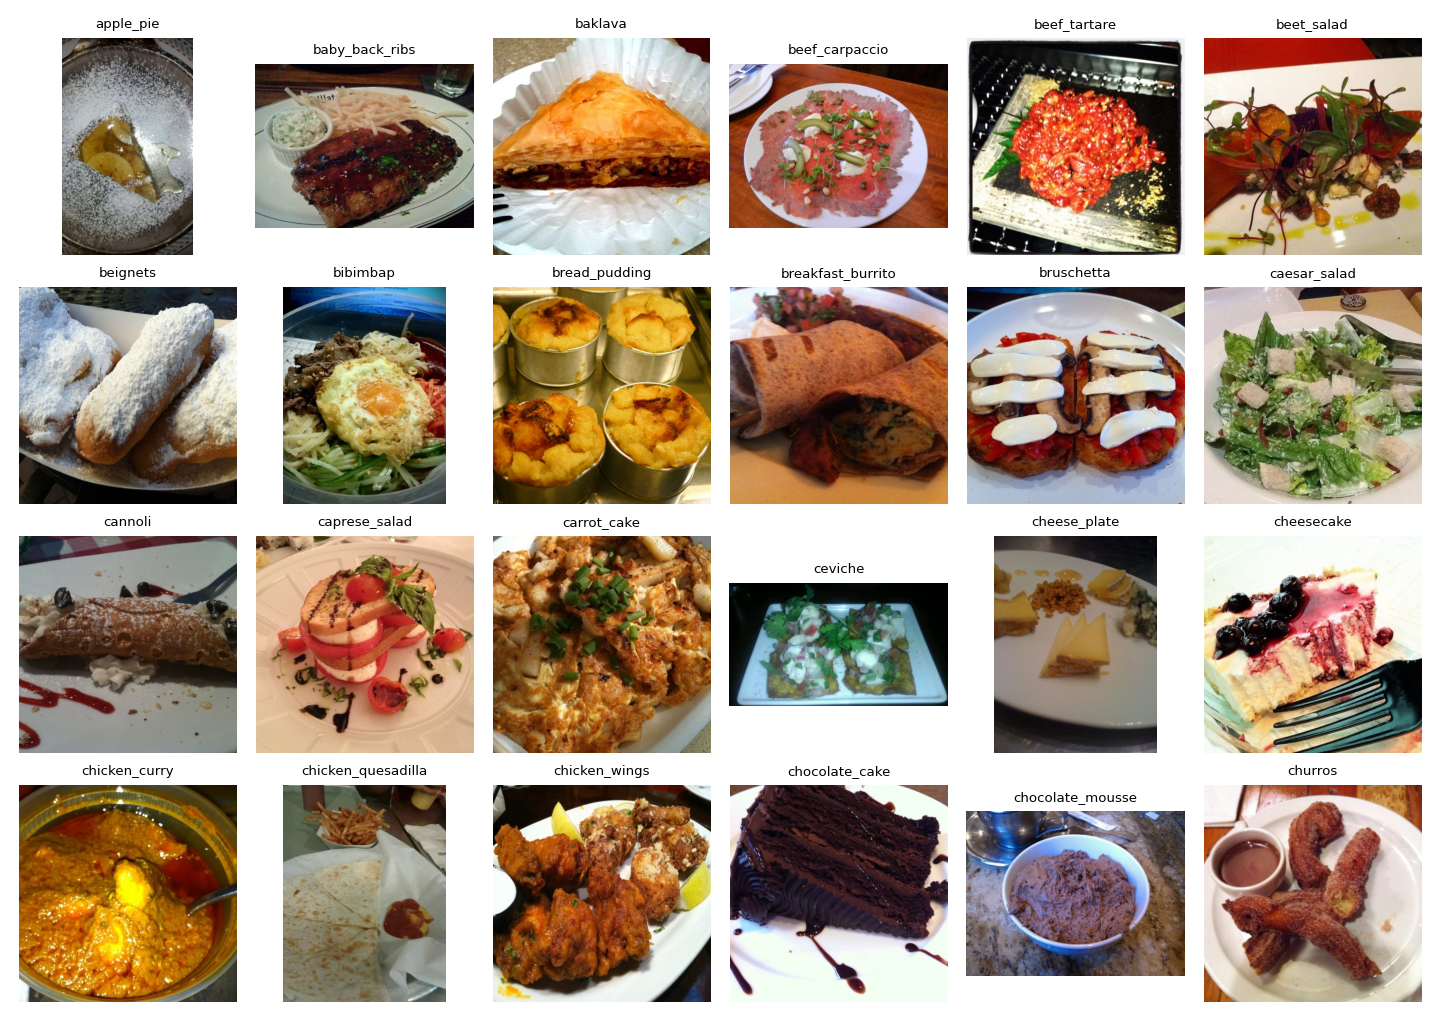
\includegraphics[width=0.85\linewidth]{samples.png}
\caption{Một ảnh mẫu (ảnh gốc) cho mỗi lớp trong 24 lớp đầu tiên.}
\label{fig:samples}
\end{figure}

\begin{figure}[H]
\centering
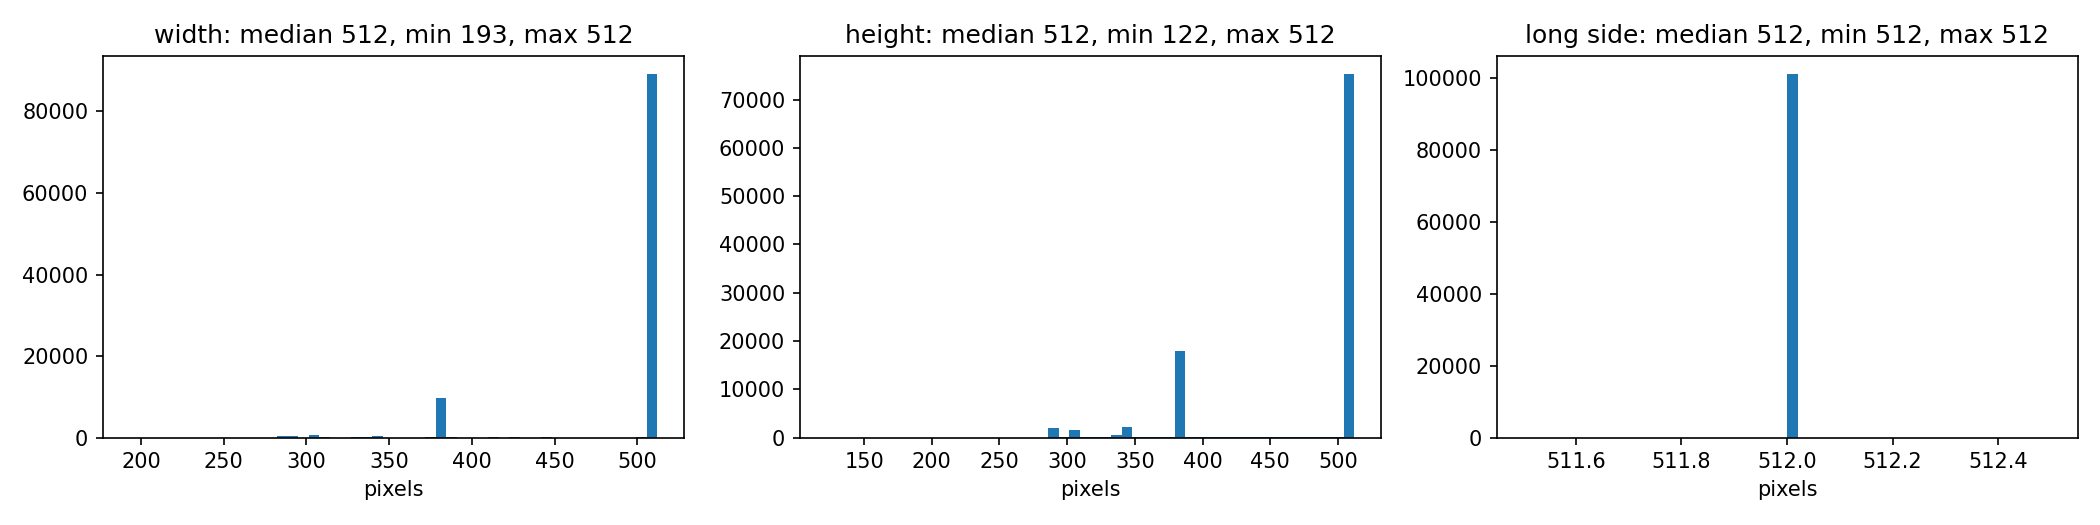
\includegraphics[width=\linewidth]{image_sizes.png}
\caption{Phân bố chiều rộng, chiều cao và cạnh dài của toàn bộ 101{,}000 ảnh.}
\label{fig:sizes}
\end{figure}

\subsection{Chia dữ liệu}
Tập test là split test chính thức và chỉ được dùng một lần ở cuối, với checkpoint có accuracy validation cao nhất. Từ split huấn luyện chính thức, chúng tôi tách 10\% ảnh của \emph{mỗi lớp} làm validation (phân tầng), dùng hoán vị \texttt{numpy.random.RandomState} với seed cố định 912 (Bảng~\ref{tab:split}, Hình~\ref{fig:classdist}). Chỉ số được lưu trong \texttt{split.npz} và dùng chung cho mọi run. Validation được dùng để chọn checkpoint và siêu tham số. Lưu ý: validation lấy từ split huấn luyện nên cũng có nhiễu nhãn, còn test thì không.

\begin{table}[H]
\centering
\caption{Chia dữ liệu Food-101 (seed chia dữ liệu $=912$).}
\label{tab:split}
\begin{tabular}{llrr}
\toprule
Tập & Nguồn & Số ảnh & Mỗi lớp \\
\midrule
Huấn luyện & split train chính thức, bỏ phần validation & 68{,}175 & 675 \\
Validation & 10\% split train chính thức, phân tầng theo lớp & 7{,}575 & 75 \\
Test & split test chính thức (đã làm sạch) & 25{,}250 & 250 \\
\bottomrule
\end{tabular}
\end{table}

\begin{figure}[H]
\centering
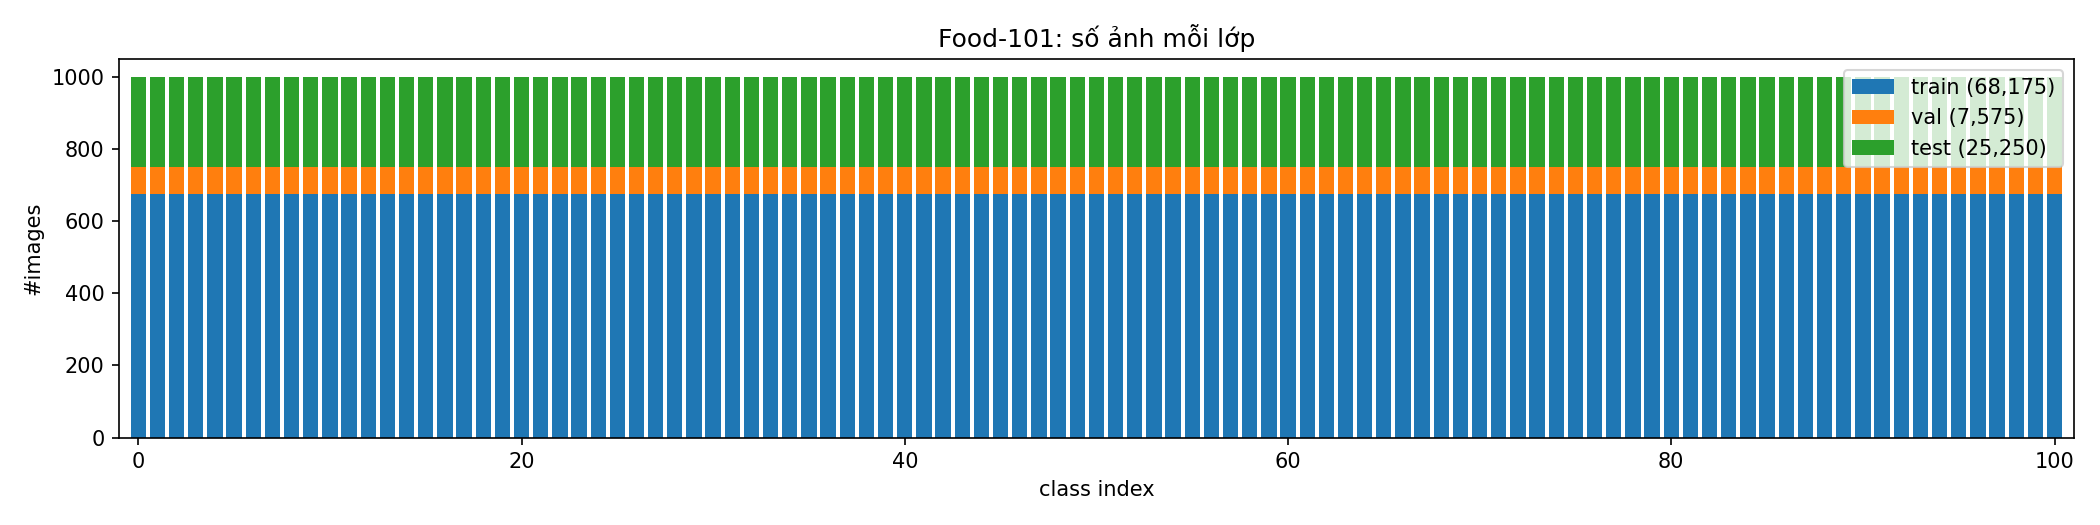
\includegraphics[width=\linewidth]{class_dist.png}
\caption{Số ảnh mỗi lớp ở ba tập; cả ba tập đều cân bằng hoàn toàn giữa các lớp.}
\label{fig:classdist}
\end{figure}

\subsection{Tiền xử lý và tăng cường dữ liệu}
Mọi ảnh được chuẩn hóa theo mean/std của ImageNet, vì các backbone pretrained được huấn luyện với chuẩn hóa này; các run from-scratch dùng cùng chuẩn hóa để mọi chế độ có cùng input.
\begin{itemize}
\item \textbf{Huấn luyện:} \texttt{RandomResizedCrop(224, scale=(0.08, 1))} $\to$ \texttt{RandomHorizontalFlip} $\to$ \texttt{TrivialAugmentWide} $\to$ chuẩn hóa.
\item \textbf{Validation / test:} \texttt{Resize(256)} $\to$ \texttt{CenterCrop(224)} $\to$ chuẩn hóa; không tăng cường.
\end{itemize}
Cùng một pipeline được dùng cho mọi run để khác biệt giữa các chế độ chỉ đến từ khởi tạo và phần được huấn luyện. Validation dùng một dataset riêng với biến đổi của eval nên không bị tăng cường. Hình~\ref{fig:aug} minh họa các biến đổi.

\begin{figure}[H]
\centering
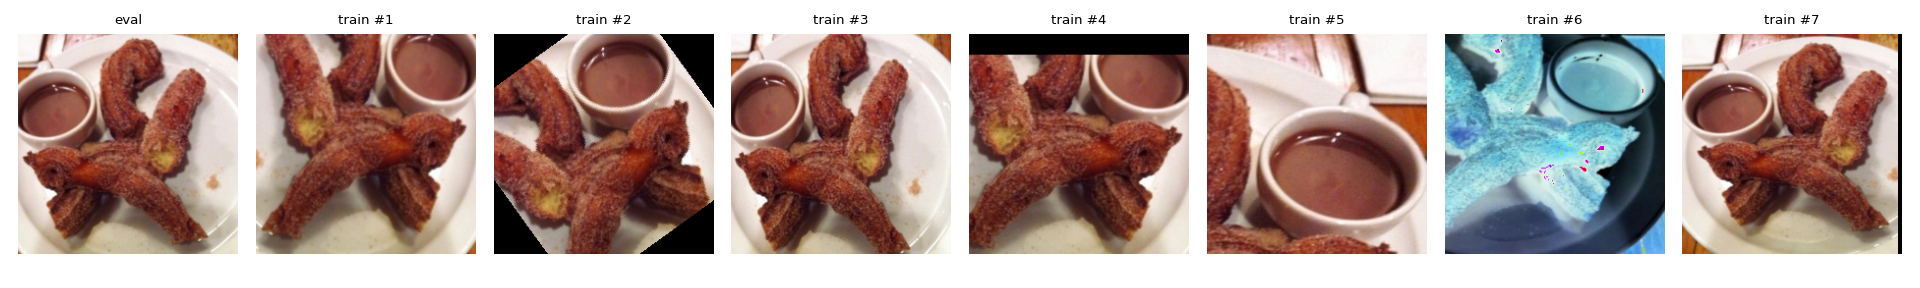
\includegraphics[width=\linewidth]{augment.png}
\caption{Một ảnh qua biến đổi eval (trái) và 7 lần lấy mẫu biến đổi huấn luyện.}
\label{fig:aug}
\end{figure}

\section{Mô hình}
Chúng tôi chọn một CNN và một Transformer có số tham số tương đương và cùng dữ liệu pretrain (ImageNet-1k), để khác biệt chủ yếu đến từ kiến trúc (Bảng~\ref{tab:models}). Trọng số pretrained lấy từ thư viện \texttt{timm}; head phân loại được thay bằng một lớp tuyến tính 101 lớp khởi tạo ngẫu nhiên.

\begin{table}[H]
\centering
\caption{Hai mô hình dùng trong A1 (số tham số tính với head 101 lớp).}
\label{tab:models}
\begin{tabular}{lllr}
\toprule
Họ & Mô hình & Trọng số pretrained (\texttt{timm}) & Tham số \\
\midrule
CNN & ResNet-50~\cite{he2016} & \texttt{resnet50.a1\_in1k} & 23{,}714{,}981 \\
Transformer & DeiT-S/16~\cite{touvron2021} & \texttt{deit\_small\_patch16\_224.fb\_in1k} & 21{,}704{,}549 \\
\bottomrule
\end{tabular}
\end{table}

\section{Protocol thí nghiệm}

\subsection{Các chế độ huấn luyện}
Mỗi mô hình được chạy ở bốn chế độ (Bảng~\ref{tab:modes}), tổng cộng 8 run. From-scratch so với full fine-tune trả lời câu hỏi pretrained giúp bao nhiêu với từng họ; ba chế độ trên bản pretrained trả lời câu hỏi nên freeze đến đâu. Với chế độ freeze một phần, chúng tôi freeze khoảng nửa đầu theo độ sâu: ResNet-50 freeze stem và \texttt{layer1}--\texttt{layer3} (64\% tham số vẫn được huấn luyện, vì \texttt{layer4} chứa phần lớn tham số), DeiT-S freeze patch embedding, positional embedding, token CLS và 6/12 block đầu (49\%). Phần bị freeze đặt \texttt{requires\_grad=False} và giữ ở chế độ \texttt{eval()}, nên BatchNorm của ResNet dùng thống kê của ImageNet và không được cập nhật.

\begin{table}[H]
\centering
\caption{Ma trận thí nghiệm và số tham số trainable.}
\label{tab:modes}
\small
\begin{tabular}{llrlr}
\toprule
Chế độ & ResNet-50: phần huấn luyện & Trainable & DeiT-S: phần huấn luyện & Trainable \\
\midrule
From-scratch & toàn bộ (khởi tạo ngẫu nhiên) & 23.71M & toàn bộ (khởi tạo ngẫu nhiên) & 21.70M \\
Freeze toàn bộ & chỉ head & 0.21M & chỉ head & 0.04M \\
Freeze một phần & \texttt{layer4} + head & 15.17M & block 7--12 + norm + head & 10.69M \\
Full fine-tune & toàn bộ & 23.71M & toàn bộ & 21.70M \\
\bottomrule
\end{tabular}
\end{table}

\subsection{Recipe huấn luyện dự kiến}
Vòng lặp huấn luyện tự viết bằng PyTorch như E1--E3. AdamW, warmup 5\% số bước rồi cosine, weight decay 0.05, batch 128, mixed precision bf16, grad clip 1.0, label smoothing 0.1. Số epoch: 15 cho freeze toàn bộ, 30 cho freeze một phần và full fine-tune, 100 cho from-scratch. Learning rate chọn trên validation; giá trị khởi điểm dự kiến là $10^{-3}$ cho chế độ chỉ train head, $10^{-4}$ (ResNet) và $5\cdot10^{-5}$ (DeiT) cho fine-tune, $10^{-3}$ (ResNet) và $5\cdot10^{-4}$ (DeiT) cho from-scratch. Cả 8 run dùng seed 912; nếu còn thời gian, 6 run pretrained (rẻ hơn nhiều) được chạy thêm với seed 42 và 100 để ước lượng độ dao động. Ước lượng khoảng 1 phút mỗi epoch trên một A100, tổng cộng khoảng 6--7 giờ GPU trên $2\times$ A100.

\subsection{Độ đo và phân tích}
\begin{itemize}
\item \textbf{Chất lượng:} accuracy top-1 và top-5, macro-F1 trên validation và test.
\item \textbf{Chi phí:} số tham số trainable, thời gian mỗi epoch, throughput (ảnh/giây) khi huấn luyện và suy luận, bộ nhớ GPU đỉnh.
\item \textbf{Lỗi:} confusion matrix 101 lớp, các cặp lớp nhầm nhiều nhất, ảnh bị sai với độ tự tin cao, các lớp có F1 thấp nhất.
\end{itemize}
Các câu hỏi sẽ trả lời ở A1.2: (1) pretrained giúp DeiT nhiều hơn ResNet bao nhiêu, do Transformer thiếu inductive bias cục bộ của convolution; (2) khi nào freeze có lợi: chỉ train head rất rẻ nhưng bị giới hạn bởi đặc trưng học từ ImageNet, còn freeze một phần có giữ được accuracy của full fine-tune với chi phí thấp hơn không; (3) đánh đổi giữa accuracy và chi phí của hai họ kiến trúc.

\begin{thebibliography}{9}
\bibitem{bossard2014} L. Bossard, M. Guillaumin, L. Van Gool. Food-101 -- Mining Discriminative Components with Random Forests. \emph{ECCV}, 2014.
\bibitem{he2016} K. He, X. Zhang, S. Ren, J. Sun. Deep Residual Learning for Image Recognition. \emph{CVPR}, 2016.
\bibitem{touvron2021} H. Touvron, M. Cord, M. Douze, F. Massa, A. Sablayrolles, H. Jégou. Training data-efficient image transformers \& distillation through attention. \emph{ICML}, 2021.
\end{thebibliography}

\end{document}
